\documentclass[10pt]{beamer}
\usepackage{../../shared/styles/custom}
\usepackage{../../shared/styles/conventions}
\setbeamertemplate{navigation symbols}{}
\newcommand{\fitpic}[1]{\begin{adjustbox}{max width=\linewidth, max totalheight=0.78\textheight}#1\end{adjustbox}}
\graphicspath{ {../assets/bias-variance/figures/} }

\title{The Bias-Variance Tradeoff: A Deep Dive}
% \date{\today}
\date{August 21, 2025}
\author{Nipun Batra and teaching staff}
\institute{IIT Gandhinagar}

\begin{document}
\maketitle

\begin{frame}{Table of Contents}
\tableofcontents
\end{frame}

\section{Understanding the Problem Setup}


\begin{frame}{The Learning Problem: A Real-World Example}
\footnotesize
\begin{definitionbox}{Our Scenario}
\raggedright
\textbf{Goal:} Predict housing prices based on house area
\end{definitionbox}

\begin{examplebox}{The True Relationship}
\raggedright
\textbf{Unknown to us:} There exists a true function $f_{\theta_{\text{true}}}$ that perfectly relates area to price:
% $$y_t = f_{\theta_{\text{true}}}(x_t)$$
$$y_t = f_{\theta_{\text{true}}}(\mathbf{x}_t)$$
\end{examplebox}
\end{frame}

\begin{frame}{The Learning Problem: A Real-World Example (contd.)}
\footnotesize
\begin{center}
\fitpic{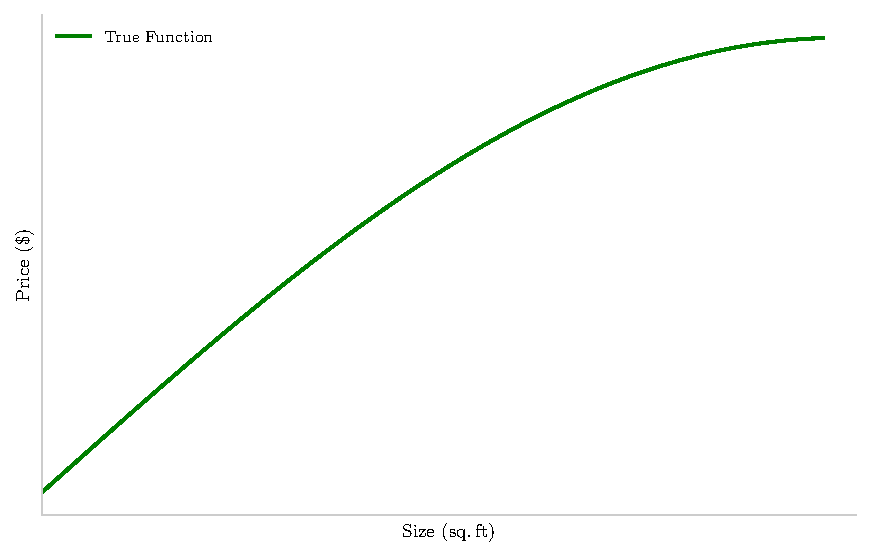
\includegraphics[width=0.65\textwidth]{../assets/bias-variance/figures/true_latexify.pdf}}
\end{center}

\begin{keypointsbox}
\raggedright
\textbf{Key Challenge:} We never know $f_{\theta_{\text{true}}}$ - we must estimate it from data!
\end{keypointsbox}
\end{frame}

\begin{frame}{The Three Sources of Prediction Error}
\footnotesize
\begin{alertbox}{Fundamental Question}
\raggedright
\textbf{Why do our predictions fail?} What causes the difference between our predictions and reality?
\end{alertbox}

\begin{definitionbox}{Three Universal Sources of Error}
\raggedright
\textbf{Every machine learning prediction suffers from:}
\begin{enumerate}
\item \textbf{Noise} - Irreducible randomness in the data
\item \textbf{Bias} - Systematic errors from model assumptions
\item \textbf{Variance} - Sensitivity to particular training sets
\end{enumerate}
\end{definitionbox}

\begin{keypointsbox}
\raggedright
\textbf{The Tradeoff:} We can often reduce bias OR variance, but not both simultaneously!
\end{keypointsbox}
\end{frame}

\begin{frame}{Preview: Error Decomposition}
\footnotesize
\begin{examplebox}{Preview}
\raggedright
\textbf{Coming up:} We'll see exactly how these three components combine mathematically and how to balance them.
\end{examplebox}
\end{frame}

\section{Source 1: Noise - The Irreducible Error}

\begin{frame}{Understanding Noise: The Fundamental Limitation}
\small
\begin{definitionbox}{What is Noise?}
\raggedright
\textbf{Noise} represents factors affecting the target that we cannot observe or control
\end{definitionbox}

\begin{examplebox}{Real-World Noise Sources}
\raggedright
\textbf{In housing prices:}
\begin{itemize}
\item House condition (hard to measure precisely)
\item Neighborhood market dynamics
\item Buyer's personal preferences
\end{itemize}
\end{examplebox}
\end{frame}

\begin{frame}{Noise: Why It's Irreducible}
\small
\begin{examplebox}{More Noise Sources}
\raggedright
\textbf{Additional factors we cannot control:}
\begin{itemize}
\item Economic conditions on sale day
\item Unmeasurable aesthetic factors
\item Random market fluctuations
\item Measurement errors in data collection
\end{itemize}
\end{examplebox}

\begin{alertbox}{Key Insight}
\raggedright
\textbf{Irreducible Error:} No matter how sophisticated our model, noise cannot be eliminated!
\end{alertbox}
\end{frame}

\begin{frame}{Noise: Mathematical Formulation}
\small
\begin{keypointsbox}{Under the Noisy conditions}
\raggedright
\textbf{True relationship becomes:}
$$y_t = f_{\theta_{\text{true}}}(x_t) + \epsilon_t$$
where $\epsilon_t \sim \mathcal{N}(0, \sigma^2)$ is the noise term
\end{keypointsbox}

\begin{center}
\fitpic{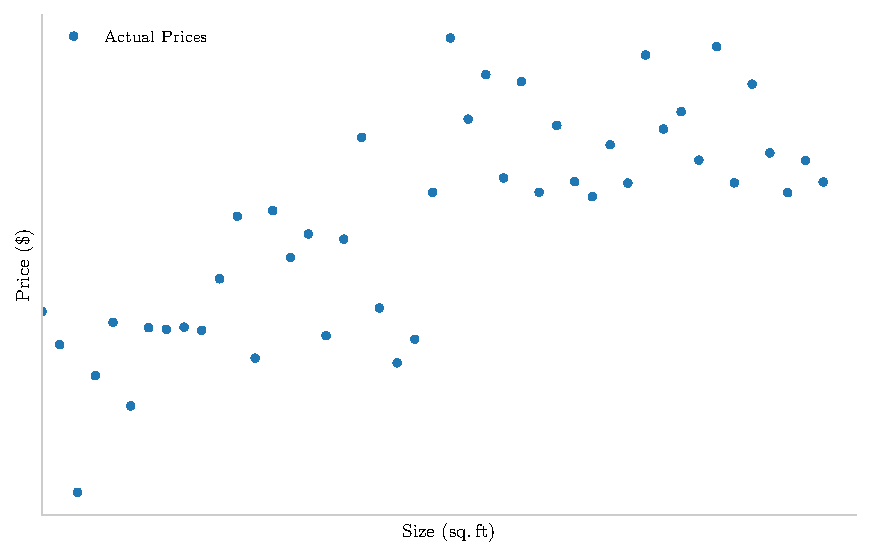
\includegraphics[width=0.65\textwidth]{../assets/bias-variance/figures/data_latexify.pdf}}
\end{center}
\end{frame}

\begin{frame}{Noise: Mathematical Properties}
\small
\begin{definitionbox}{Key Properties of Noise}
\raggedright
\begin{itemize}
\item \textbf{Zero mean:} $E[\epsilon_t] = 0$ (unbiased)
\item \textbf{Constant variance:} $\text{Var}(\epsilon_t) = \sigma^2$
\item \textbf{Independent:} Each observation's noise is independent
\end{itemize}
\end{definitionbox}

\begin{keypointsbox}{Why These Properties Matter}
\raggedright
\begin{itemize}
\item \textbf{Zero mean:} Noise doesn't systematically bias our target
\item \textbf{Constant variance:} Prediction uncertainty is consistent
\item \textbf{Independence:} One data point's noise doesn't affect others
\end{itemize}
\end{keypointsbox}
\end{frame}


\begin{frame}{Visualizing Noise: Data Distribution}
\footnotesize
\begin{center}
\fitpic{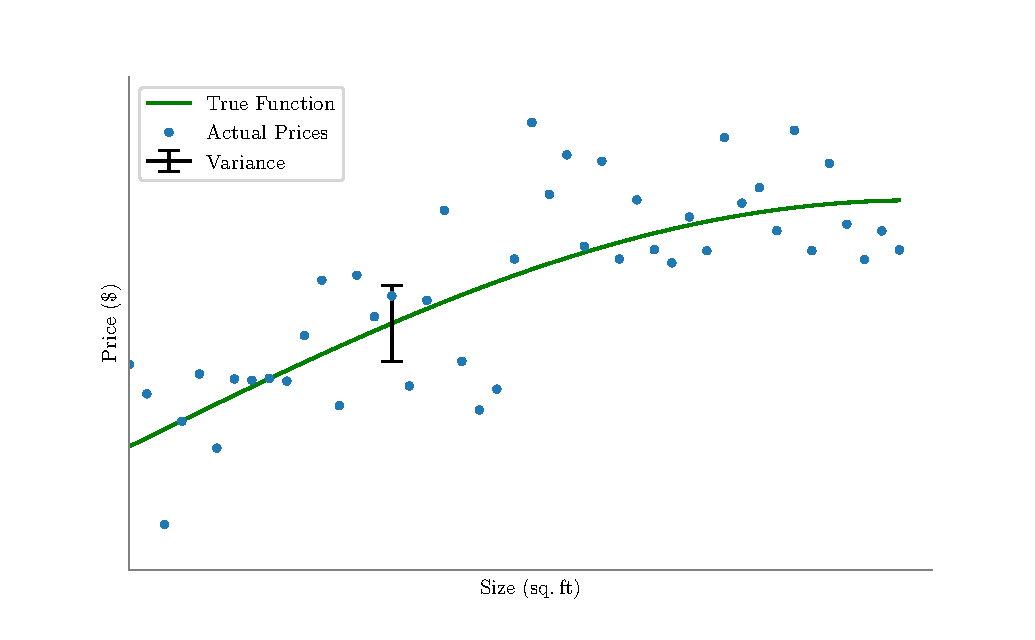
\includegraphics[width=0.75\textwidth]{../assets/bias-variance/figures/data_var_latexify.pdf}}
\end{center}
\end{frame}

\begin{frame}{Visualizing Noise: Data Distribution (contd.)}
\footnotesize
\begin{keypointsbox}
\raggedright
\textbf{Key Observation:} 
\begin{itemize}
\item Data points scatter around the true function
\item The spread (variance) is constant: $\sigma^2$
\item This randomness cannot be removed by better modeling
\end{itemize}
\end{keypointsbox}

\begin{alertbox}{Implication for ML}
\raggedright
\textbf{Lower bound on error:} Any model will have at least $\sigma^2$ error due to noise
\end{alertbox}
\end{frame}

\section{Source 2: Bias - Systematic Model Limitations}

\begin{frame}{Understanding Bias: Model Flexibility}
\small
\begin{definitionbox}{What is Bias?}
\raggedright
\textbf{Bias} measures how well our model class can represent the true function
\end{definitionbox}

\begin{examplebox}{Extreme Example: Constant Function}
\raggedright
\textbf{Model choice:} $\hat{f}(x) = c$ (constant, regardless of house size)

\textbf{Question:} Can this model capture the true price-size relationship?
\end{examplebox}
\end{frame}

\begin{frame}{Bias: Visualizing the Problem}
\begin{center}
\fitpic{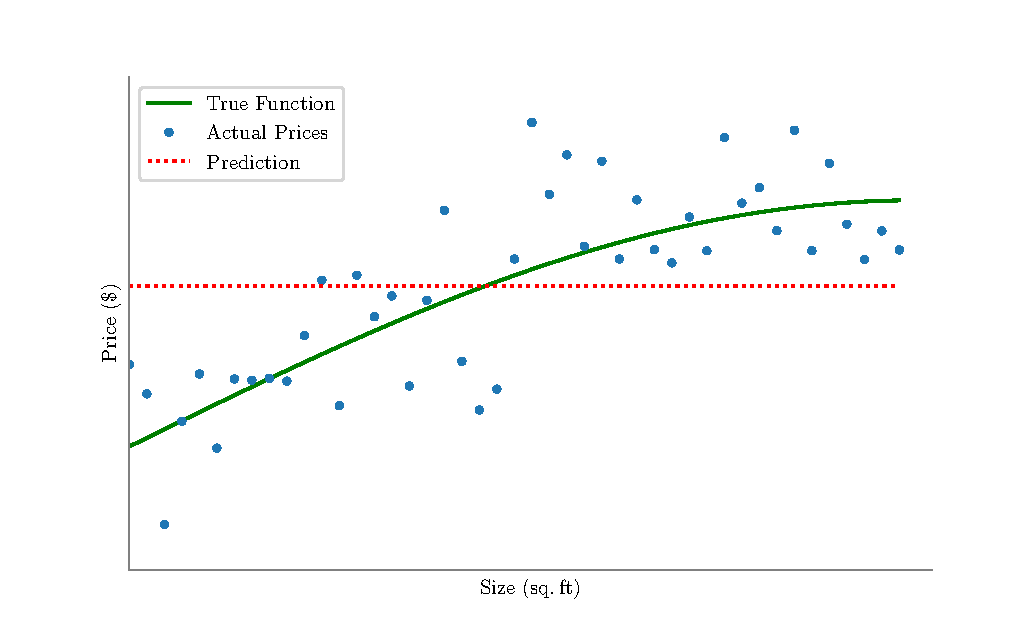
\includegraphics[width=0.75\textwidth]{../assets/bias-variance/figures/biasn_2_latexify.pdf}}
\end{center}

\begin{alertbox}
\raggedright
\textbf{Obvious Problem:} A constant function cannot capture any relationship with house size!
\end{alertbox}
\end{frame}


% \begin{frame}{Bias: Fitting a Constant Model}
% \footnotesize
% \begin{center}
% \fitpic{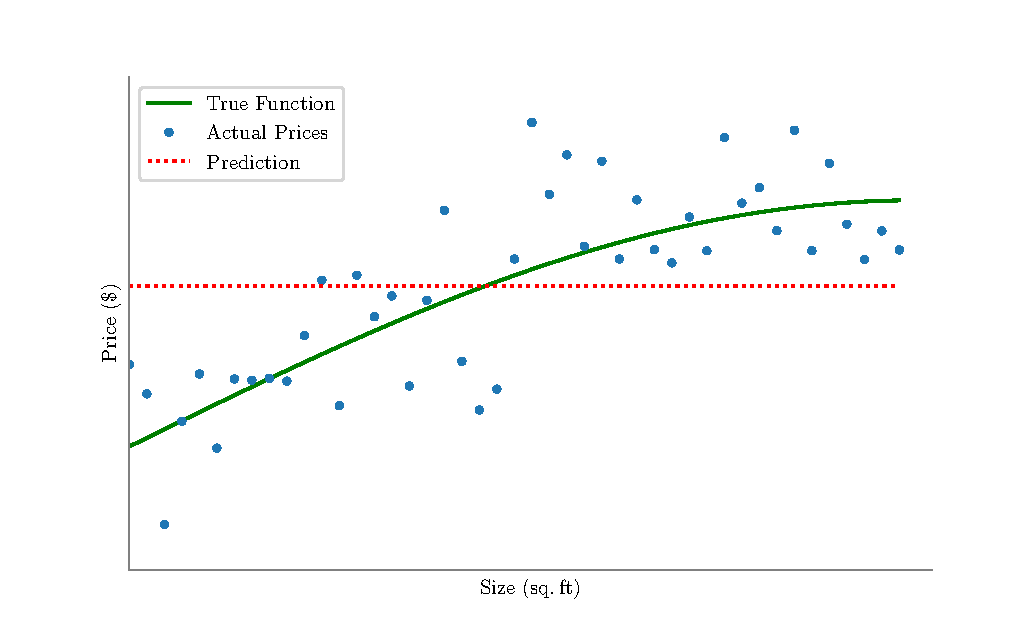
\includegraphics[width=0.75\textwidth]{../assets/bias-variance/figures/biasn_2_latexify.pdf}}
% \end{center}
% \end{frame}

\begin{frame}{Bias: Fitting a Constant Model (contd.)}
\footnotesize
\begin{keypointsbox}
\raggedright
\textbf{Best Constant Fit:} 
\begin{itemize}
\item The optimal constant is the average of all prices
\item But this completely ignores the size information!
\item Large systematic errors remain
\end{itemize}
\end{keypointsbox}
\end{frame}


\begin{frame}{Bias: Visualizing the Systematic Error}
\footnotesize
\begin{center}
\fitpic{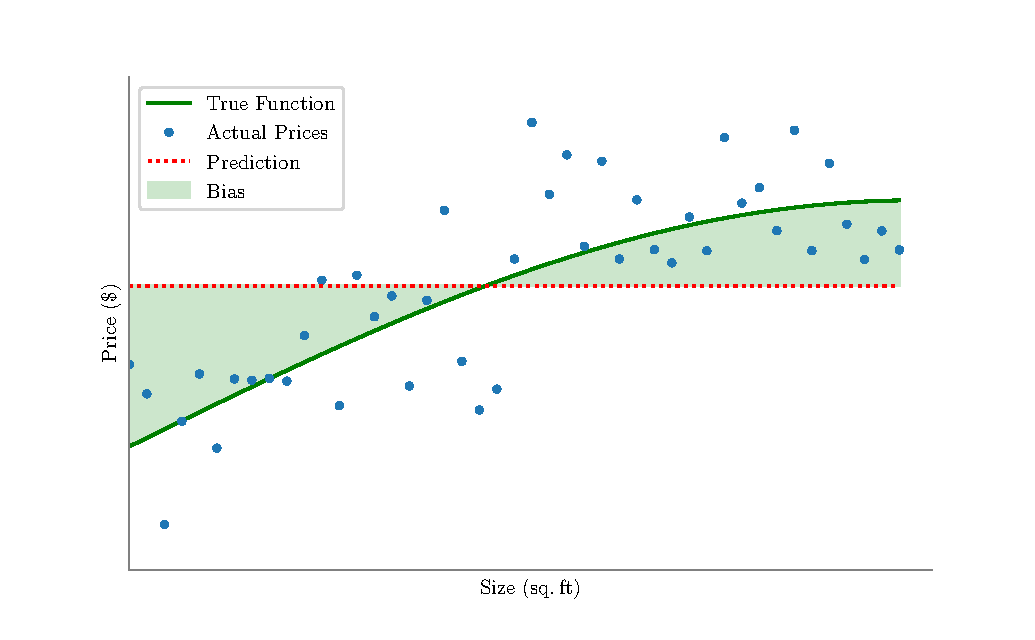
\includegraphics[width=0.7\textwidth]{../assets/bias-variance/figures/biasn_3_latexify.pdf}}
\end{center}
\end{frame}

\begin{frame}{Bias: Visualizing the Systematic Error (contd.)}
\footnotesize
\begin{definitionbox}{Bias Definition}
\raggedright
$$\text{Bias}(x) = f_{\theta_{\text{true}}}(x) - E[\hat{f}(x)]$$
The systematic difference between truth and average prediction
\end{definitionbox}

\begin{alertbox}{Key Insight}
\raggedright
\textbf{High bias = Underfitting:} Model assumptions are too restrictive
\end{alertbox}
\end{frame}



\begin{frame}{Multiple Datasets: Understanding Variability}
\footnotesize
\begin{keypointsbox}
\raggedright
\textbf{Crucial Insight:} Many different datasets are possible from the same true relationship!
\end{keypointsbox}

\begin{center}
\fitpic{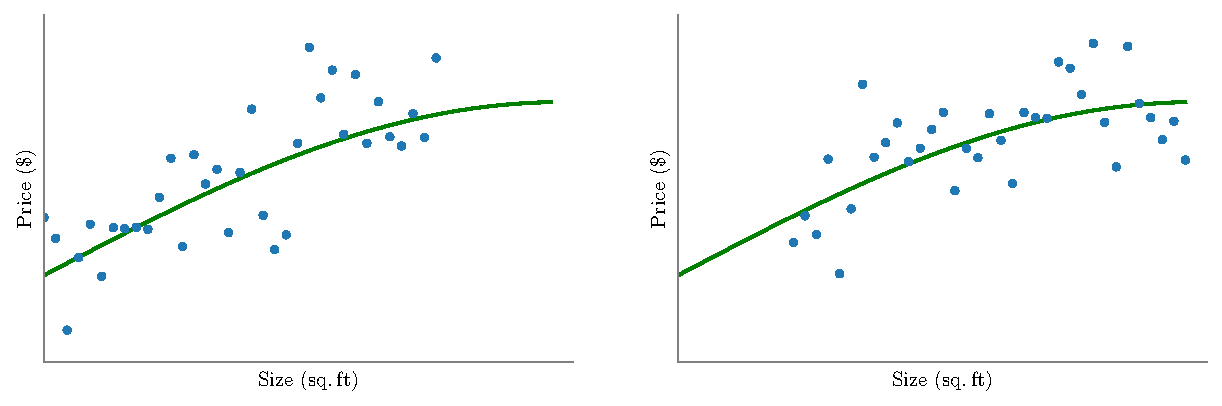
\includegraphics[width=0.9\textwidth]{../assets/bias-variance/figures/bias1_latexify.pdf}}
\end{center}
\end{frame}

\begin{frame}{Why Datasets Differ}
\footnotesize
\begin{examplebox}
\raggedright
\textbf{Same underlying relationship, different data points due to:}
\begin{itemize}
\item Random sampling of houses
\item Different noise realizations
\item Natural variation in the population
\end{itemize}
\end{examplebox}
\end{frame}

\begin{frame}{Fitting Models to Different Datasets}
\begin{center}
\fitpic{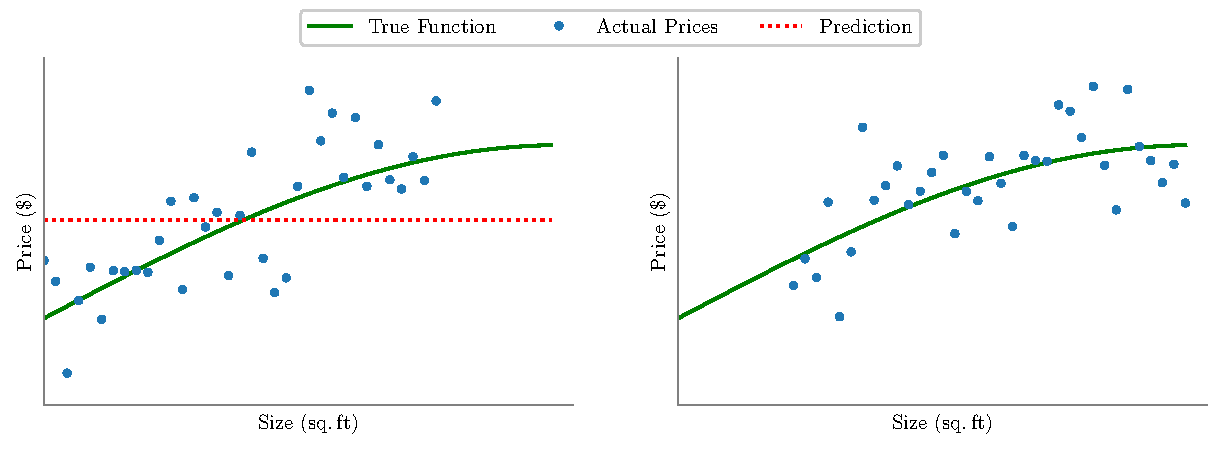
\includegraphics[width=0.9\textwidth]{../assets/bias-variance/figures/bias2_latexify.pdf}}
\end{center}

\begin{keypointsbox}
\raggedright
\textbf{Question:} If we fit the same model type (constant) to different datasets, what happens?
\end{keypointsbox}
\end{frame}


\begin{frame}{Different Predictions from Different Datasets}
\footnotesize
\begin{center}
\fitpic{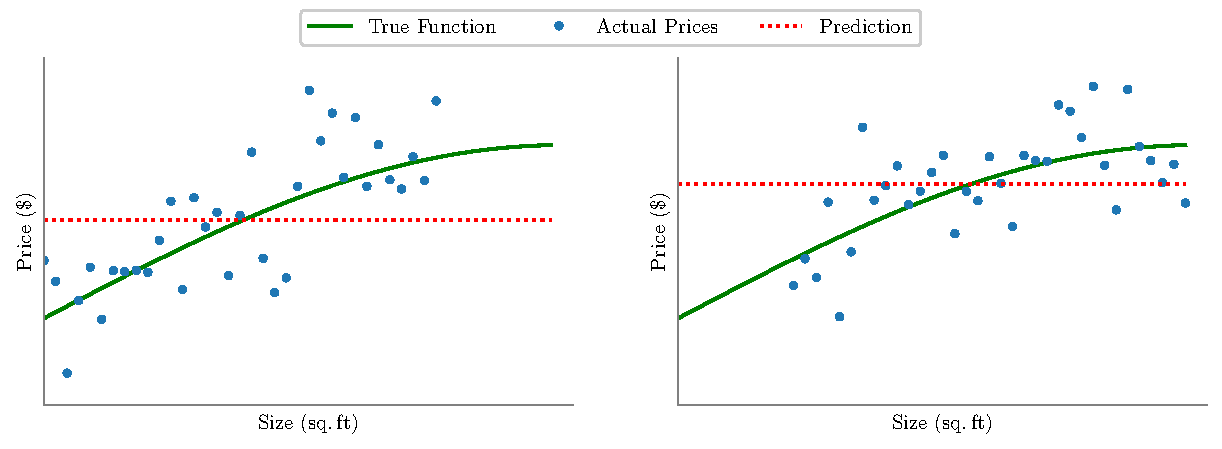
\includegraphics[width=0.9\textwidth]{../assets/bias-variance/figures/bias3_latexify.pdf}}
\end{center}

\begin{alertbox}
\raggedright
\textbf{Key Observation:} Even with the same model type, we get different predictions!
\end{alertbox}
\end{frame}

\begin{frame}{Prediction Variability: Concepts}
\footnotesize
\begin{definitionbox}
\raggedright
\textbf{This variability leads us to two concepts:}
\begin{itemize}
\item \textbf{Average prediction:} What happens "on average" across all possible datasets
\item \textbf{Prediction variance:} How much predictions vary across datasets
\end{itemize}
\end{definitionbox}
\end{frame}

\begin{frame}{Many Datasets: The Full Picture}
\footnotesize
\begin{center}
\fitpic{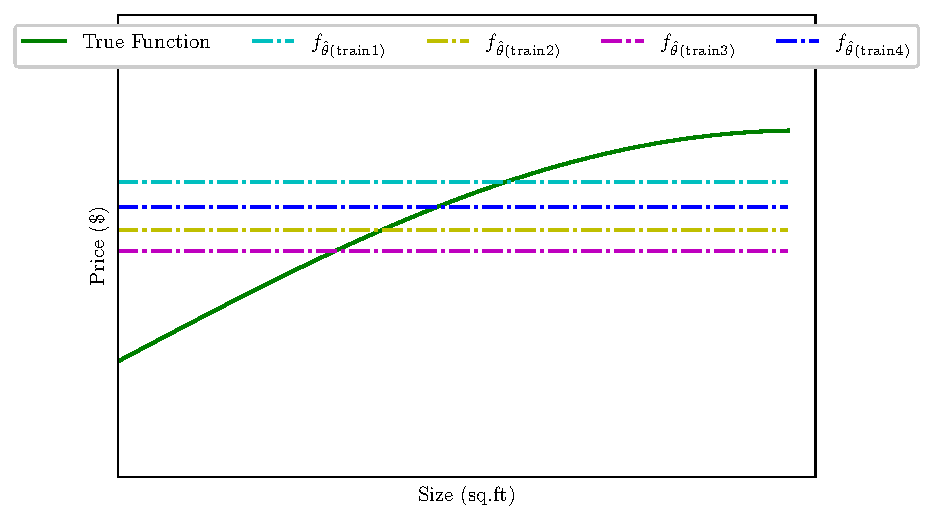
\includegraphics[width=0.75\textwidth]{../assets/bias-variance/figures/bias4_latexify.pdf}}
\end{center}

\begin{keypointsbox}
\raggedright
\textbf{Multiple Datasets:} Each gives a slightly different constant fit
\end{keypointsbox}
\end{frame}

\begin{frame}{Expected Prediction: The Big Question}
\footnotesize
\begin{examplebox}
\raggedright
\textbf{The Big Question:} What is the "typical" or "expected" prediction our model makes?
\end{examplebox}
\end{frame}

\begin{frame}{The Average Model: Expected Prediction}
\footnotesize
\begin{center}
\fitpic{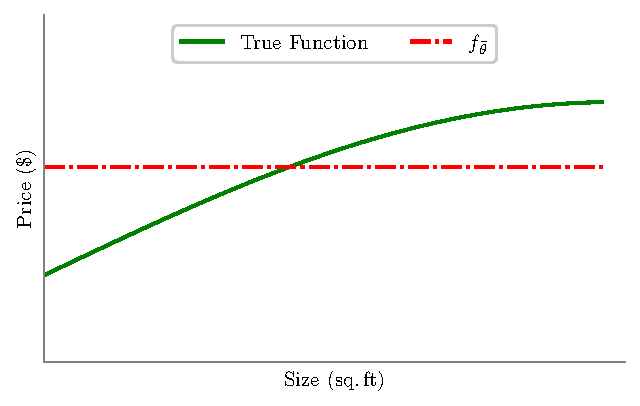
\includegraphics[width=0.65\textwidth]{../assets/bias-variance/figures/bias5_latexify.pdf}}
\end{center}
\end{frame}

\begin{frame}{Expected Prediction: Definition}
\footnotesize
\begin{definitionbox}{Expected Prediction}
\raggedright
$$E[\hat{f}(x)] = \text{Average prediction across all possible training sets}$$
\end{definitionbox}

\begin{keypointsbox}
\raggedright
\textbf{For constant models:} The expected prediction is the expected value of the target variable
\end{keypointsbox}
\end{frame}


\begin{frame}{Bias: The Final Definition}
\small
\begin{definitionbox}{Bias Formula}
\raggedright
$$\text{Bias}(x) = f_{\theta_{\text{true}}}(x) - E[\hat{f}(x)]$$
\textbf{Difference between truth and expected prediction}
\end{definitionbox}

\begin{center}
\fitpic{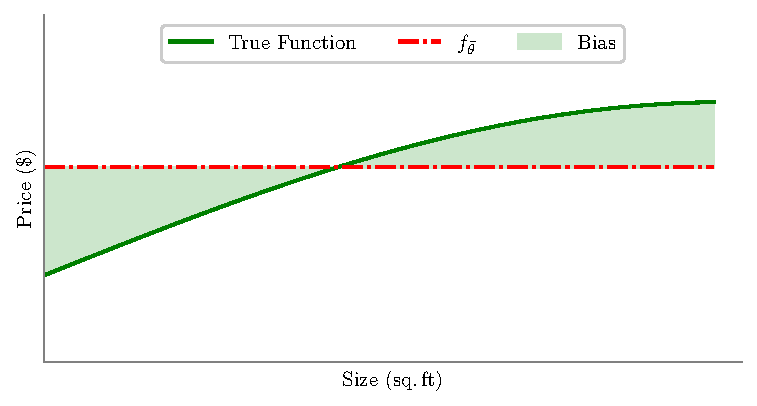
\includegraphics[width=0.65\textwidth]{../assets/bias-variance/figures/bias6_latexify.pdf}}
\end{center}
\end{frame}

\begin{frame}{Model Complexity vs Bias: The Relationship}
\begin{keypointsbox}
\textbf{Universal Pattern:} As model complexity increases, model become flexible enough  to  approximate true function , hence  bias decreases

\end{keypointsbox}

\begin{center}
\fitpic{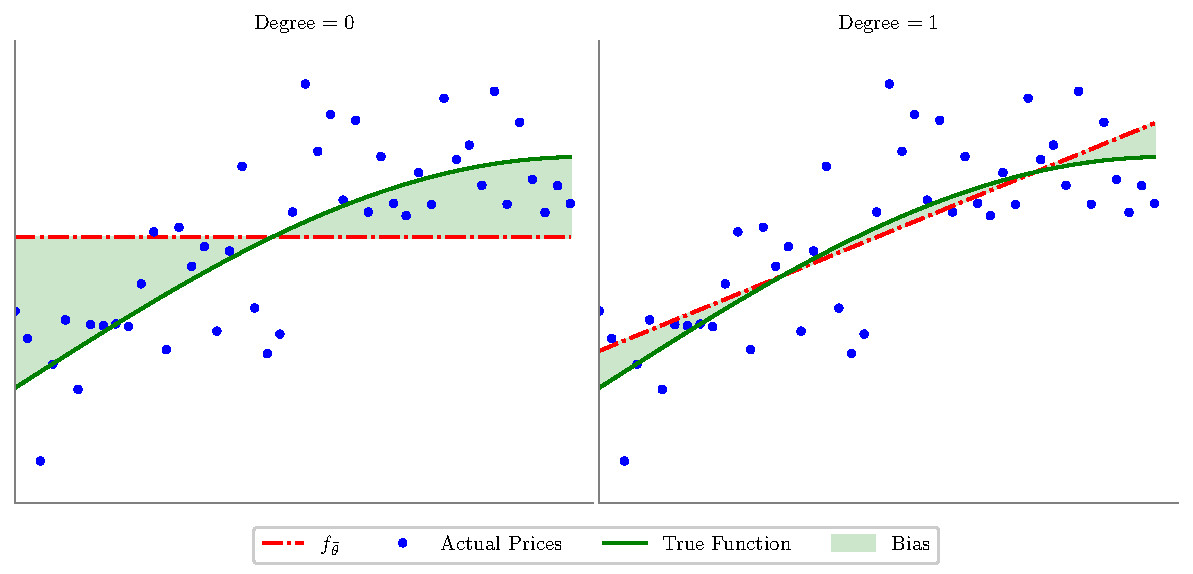
\includegraphics[width=0.95\textwidth]{../assets/bias-variance/figures/bias7_latexify.pdf}}
\end{center}


\end{frame}

\section{Variance: Sensitivity to Data}

\begin{frame}{From Bias to Variance: The Other Side}
\begin{alertbox}
\textbf{We've seen:} High-complexity models have low bias

\textbf{Question:} If low bias is good, why not always use high-complexity models?
\end{alertbox}

\begin{definitionbox}{Enter Variance}
\textbf{Variance} measures how much predictions change when we train on different datasets
\end{definitionbox}

\begin{keypointsbox}
\textbf{Intuition:} Simple models  are Stable, consistent predictions, while Complex models are highly sensitive to specific training data

\end{keypointsbox}


\end{frame}

\begin{frame}{Understanding Variance: Prediction Consistency}
\begin{definitionbox}{Variance Definition}
\textbf{Variance} = How much do predictions vary across different training sets?
$$\text{Var}(\hat{f}(x)) = E[(\hat{f}(x) - E[\hat{f}(x)])^2]$$
\end{definitionbox}

\begin{center}
\fitpic{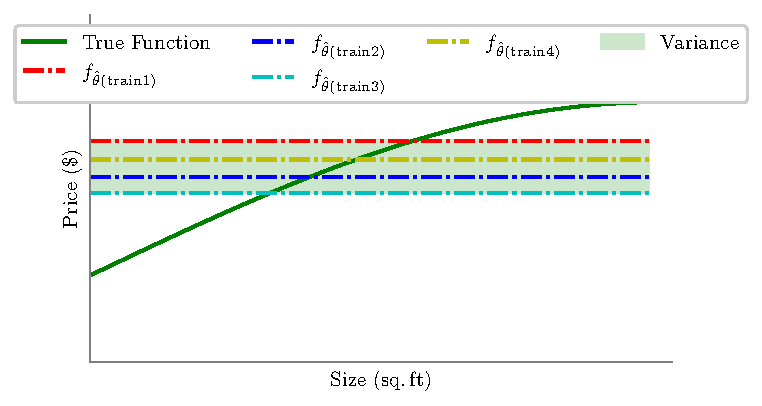
\includegraphics[width=0.7\textwidth]{../assets/bias-variance/figures/var1_latexify.pdf}}
\end{center}


\end{frame}

\begin{frame}{Low Complexity: Low Variance}
\begin{keypointsbox}
\textbf{Simple Models (e.g., linear):} Simple model have few parameters to estimate which leads to consistent predictions across different training sets.

\end{keypointsbox}

\begin{center}
\fitpic{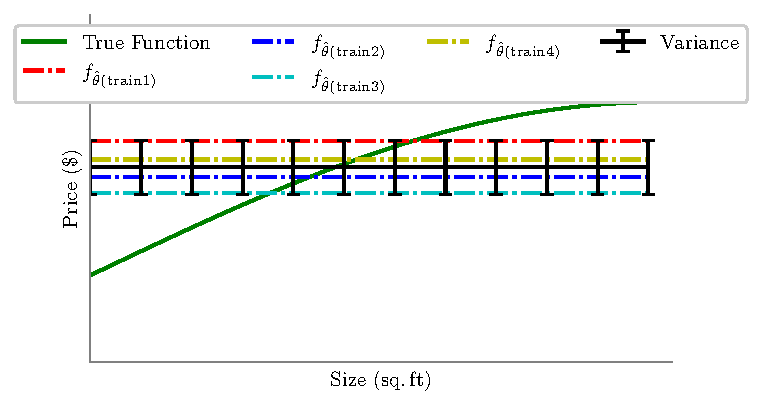
\includegraphics[width=0.7\textwidth]{../assets/bias-variance/figures/var2_latexify.pdf}}
\end{center}

% \begin{definitionbox}
% \textbf{Low Variance = Stability:} Predictions don't change much with different training sets
% \end{definitionbox}
\end{frame}

\begin{frame}{High Complexity: The Variance Problem Emerges}
\begin{center}
\fitpic{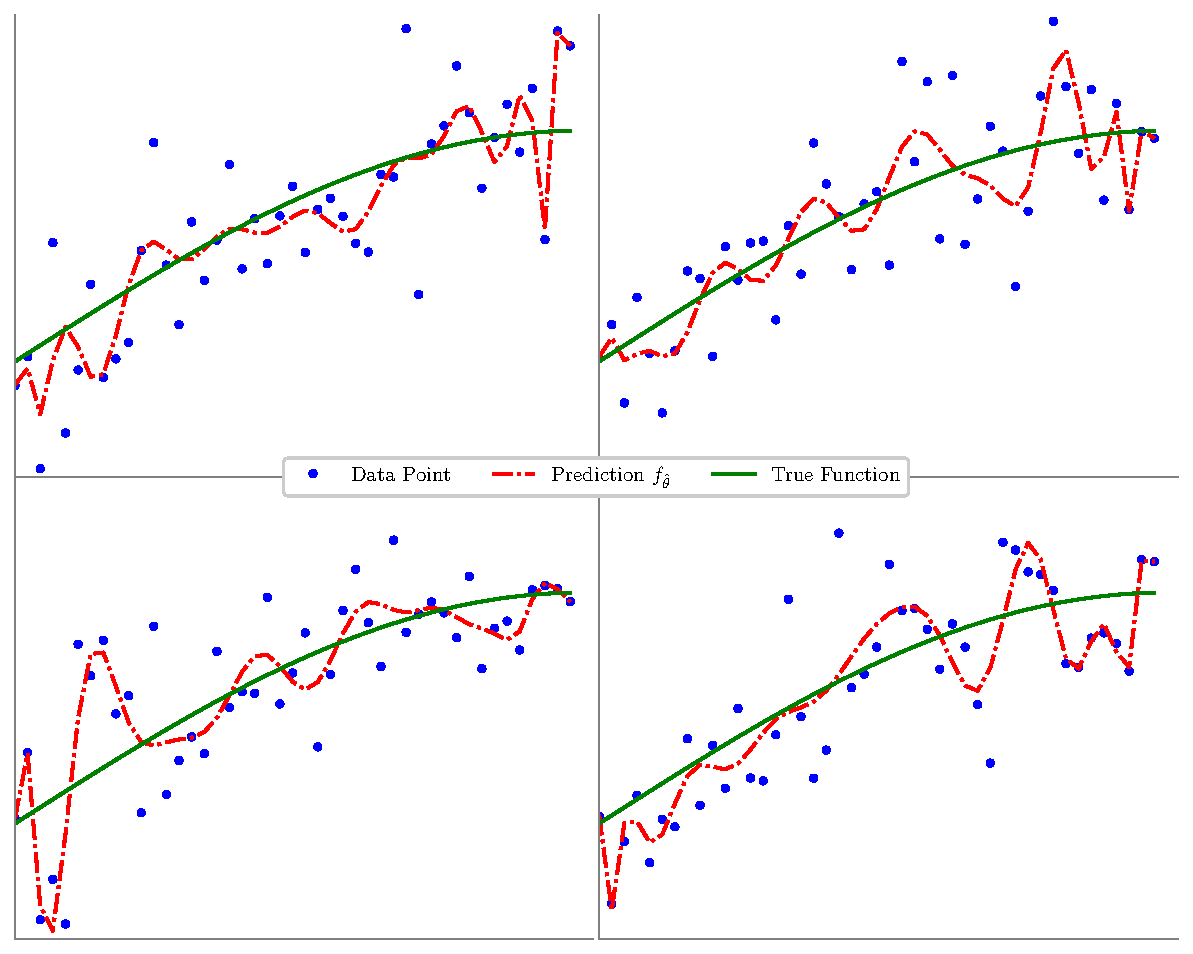
\includegraphics[width=0.7\textwidth]{../assets/bias-variance/figures/var3_latexify.pdf}}
\end{center}


\end{frame}

\begin{frame}{High Complexity: Extreme Variance}
\begin{keypointsbox}
\textbf{Complex Models (e.g., high-degree polynomials):} Complex models have  many parameters to estimate which leads to dramatic different predictions across different training sets.

\end{keypointsbox}

\begin{center}
\fitpic{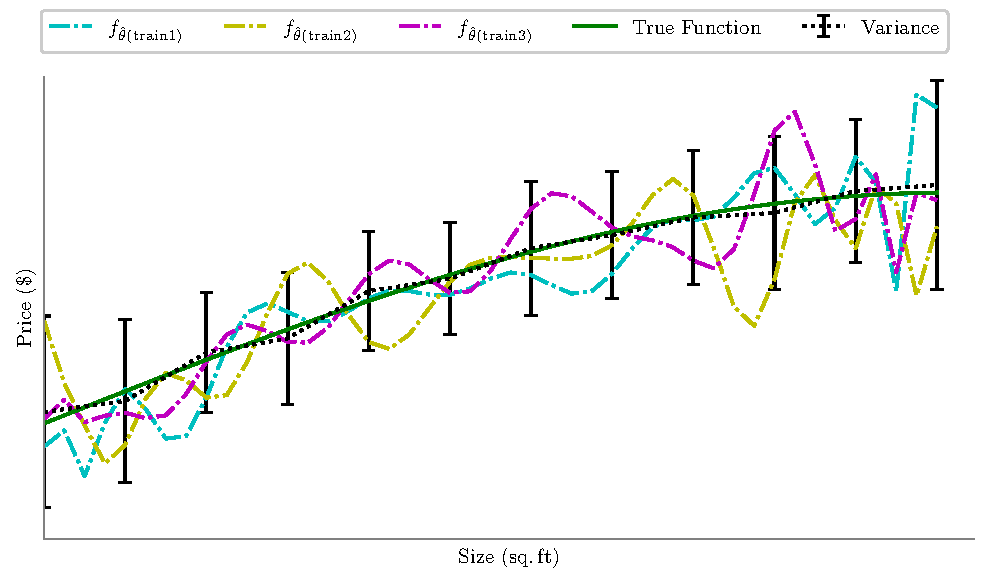
\includegraphics[width=0.8\textwidth]{../assets/bias-variance/figures/var4_latexify.pdf}}
\end{center}

\begin{alertbox}
\textbf{High Variance = Overfitting:} Model memorizes training data instead of learning general patterns
\end{alertbox}
\end{frame}

\begin{frame}{The Bias-Variance Tradeoff: The Central Tension}
\begin{center}
\fitpic{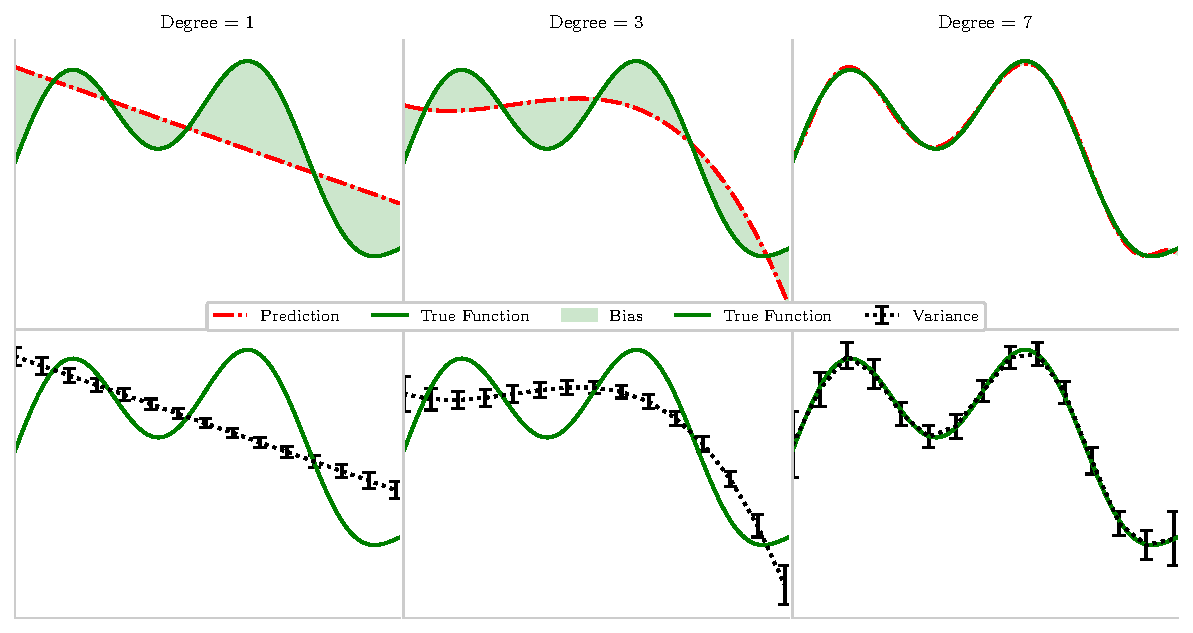
\includegraphics[width=0.95\textwidth]{../assets/bias-variance/figures/bv-2_latexify.pdf}}
\end{center}
\end{frame}
\begin{frame}{The Bias-Variance Tradeoff: The Central Tension}
\begin{alertbox}{The Fundamental Tradeoff}
\begin{itemize}
\item \textbf{Simple models:} High bias, low variance
\item \textbf{Complex models:} Low bias, high variance
\item \textbf{Optimal complexity:} Balance between the two
\end{itemize}
\end{alertbox}

\begin{keypointsbox}
\textbf{Key Insight:} We cannot minimize both bias and variance simultaneously!
\end{keypointsbox}
\end{frame}


\section{Mathematical Decomposition}

\begin{frame}{Why Mathematical Analysis Matters}
\small

\begin{definitionbox}{The Goal}
\raggedright
Can we mathematically prove that prediction error can be expressed as a function of bias, variance, and noise?\\[1ex]
Specifically, can we show:
$$
\text{error}= E\left[(y - \hat{f}(x))^2\right] = \text{function of bias, variance, and noise}
$$
\end{definitionbox}

\begin{keypointsbox}{Why This Matters}
\raggedright
\begin{itemize}
\item Understand the fundamental limits of learning
\item Make informed model and algorithm choices
\item Explicitly balance bias and variance
\end{itemize}
\end{keypointsbox}


\end{frame}

\begin{frame}{Bias-Variance Decomposition: The Goal}
\small
\begin{definitionbox}{What We Want to Prove}
\raggedright
% $$E[(y - \hat{f}(x))^2] = \text{Noise} + \text{Bias}^2 + \text{Variance}$$
$$
\text{error}= E\left[(y - \hat{f}(x))^2\right] = \text{function of bias, variance, and noise}
$$
\end{definitionbox}



\begin{keypointsbox}{Strategy}
\raggedright
\begin{enumerate}
\item Start with squared error at a single point
\item Take expectation over all randomness (training set and noise)
\item Use algebraic tricks to separate terms
\item Identify noise, bias, and variance
\end{enumerate}
\end{keypointsbox}
\end{frame}

\begin{frame}{Step 1: The Squared Error}
\small
\begin{definitionbox}{Squared Loss at $x$}
\raggedright
\textbf{Prediction error:} $(y - \hat{f}(x))^2$
\end{definitionbox}

\begin{keypointsbox}{Taking Expectations}
\raggedright
\textbf{Expected error:}
$$E_{\mathcal{D}, y}[(y - \hat{f}(x))^2]$$
where:
\begin{itemize}
\item $\mathcal{D}$: Random training set
\item $y$: Random target (includes noise)
\end{itemize}
\end{keypointsbox}
\end{frame}

\begin{frame}{Step 2: Add and Subtract the True Function}
\small
\begin{examplebox}{The Trick}
\raggedright
Add and subtract $f_{\text{true}}(x)$ inside the square:
$$E[(y - f_{\text{true}}(x) + f_{\text{true}}(x) - \hat{f}(x))^2]$$
\end{examplebox}

\begin{keypointsbox}{Earlier seen : Under Noisy conditions}
\raggedright
\textbf{True relationship becomes:}
$$y_t = f_{\theta_{\text{true}}}(x_t) + \epsilon_t$$
\end{keypointsbox}
\begin{definitionbox}{Grouping Terms}
\raggedright
$$E\left[\underbrace{(y - f_{\text{true}}(x))}_{\epsilon} + \underbrace{(f_{\text{true}}(x) - \hat{f}(x))}_{\text{prediction error}}\right]^2$$
\end{definitionbox}
\end{frame}

\begin{frame}{Step 3: Expand the Square}
\small
\begin{examplebox}{Algebraic Expansion}
\raggedright
Let $a = \epsilon$, $b = f_{\text{true}}(x) - \hat{f}(x)$:
$$(a + b)^2 = a^2 + 2ab + b^2$$
So,
$$E[\epsilon^2 + 2\epsilon(f_{\text{true}}(x) - \hat{f}(x)) + (f_{\text{true}}(x) - \hat{f}(x))^2]$$
\end{examplebox}

\begin{keypointsbox}{Linearity of Expectation}
\raggedright
$$E[\epsilon^2] + 2E[\epsilon(f_{\text{true}}(x) - \hat{f}(x))] + E[(f_{\text{true}}(x) - \hat{f}(x))^2]$$
\end{keypointsbox}
\end{frame}

\begin{frame}{Step 4: Identify the Three Terms}
\small
\begin{definitionbox}{Three Terms}
\raggedright
\begin{itemize}
\item \textbf{Term 1:} $E[\epsilon^2]$ (noise)
\item \textbf{Term 2:} $2E[\epsilon(f_{\text{true}}(x) - \hat{f}(x))]$ (cross-term)
\item \textbf{Term 3:} $E[(f_{\text{true}}(x) - \hat{f}(x))^2]$ (prediction error)
\end{itemize}
\end{definitionbox}

\begin{keypointsbox}{Next Steps}
\raggedright
Analyze each term separately to reveal noise, bias, and variance.
\end{keypointsbox}
\end{frame}

% --- Term 1: Noise ---
% \begin{frame}{Step 5: Analyzing Term 1 (Noise)}
% \small
% \begin{definitionbox}{Term 1}
% \raggedright
% $\epsilon = y - f_{\text{true}}(x)$ is the noise.\\
% \textbf We know that {Variance}  is defined as:
% $$\text{Var}(\epsilon^2) = E[\epsilon^2] - (E[\epsilon])^2 $$ ,so here in this case, we can write:
% $E[\epsilon^2] = \text{Var}(\epsilon) + (E[\epsilon])^2 = \sigma^2 + 0^2 = \sigma^2$
% \end{definitionbox}
\begin{frame}{Step 5: Analyzing Term 1 (Noise)}
\small
\begin{definitionbox}{Term 1}
\raggedright
$\epsilon = y - f_{\text{true}}(x)$ is the noise.\\[1ex]
\textbf{Recall how variance is defined:}
\begin{align*}
\text{Var}(\epsilon)
&= \mathbb{E}\left[(\epsilon - \mathbb{E}[\epsilon])^2\right] \\[6pt]
&= \mathbb{E}\left[\epsilon^2 - 2\epsilon \, \mathbb{E}[\epsilon] + (\mathbb{E}[\epsilon])^2\right] \\[6pt]
&= \mathbb{E}[\epsilon^2] - 2\mathbb{E}[\epsilon]\mathbb{E}[\epsilon] + (\mathbb{E}[\epsilon])^2 \\[6pt]
&= \mathbb{E}[\epsilon^2] - (\mathbb{E}[\epsilon])^2
\end{align*}
So, \(\mathbb{E}[\epsilon^2] = \text{Var}(\epsilon) + \left(\mathbb{E}[\epsilon]\right)^2\). 
\\For our noise, \(\mathbb{E}[\epsilon] = 0\) and \(\text{Var}(\epsilon) = \sigma^2\), so 
\(\mathbb{E}[\epsilon^2] = \sigma^2 + 0^2 = \sigma^2\).
 
$\boxed{\text{Term 1} = \sigma^2}$, \textbf{This is the irreducible error (noise)!}
\end{definitionbox}

% \begin{alertbox}{Result}
% \raggedright
% $\boxed{\text{Term 1} = \sigma^2}$, \textbf{This is the irreducible error (noise)!}
% \end{alertbox}
\end{frame}

% \begin{alertbox}{Result}
% \raggedright
% $\boxed{\text{Term 1} = \sigma^2}$\\
% \textbf{This is the irreducible error (noise)!}
% \end{alertbox}
% \end{frame}

% --- Term 2: Cross-term ---
\begin{frame}{Step 6: Analyzing Term 2 (Cross-Term)}
\small
\begin{definitionbox}{Term 2}
\raggedright
$2E[\epsilon(f_{\text{true}}(x) - \hat{f}(x))]$
\end{definitionbox}

\begin{keypointsbox}{Key Insight}
\raggedright
$\epsilon$ (noise) is independent of $\hat{f}(x)$ (model prediction), so:
$$E[\epsilon(f_{\text{true}}(x) - \hat{f}(x))] = E[\epsilon] \cdot E[f_{\text{true}}(x) - \hat{f}(x)] = 0$$
\end{keypointsbox}

\begin{alertbox}{Result}
\raggedright
$\boxed{\text{Term 2} = 0}$\\
\textbf{The cross-term vanishes!}
\end{alertbox}
\end{frame}

% --- Term 3: Prediction Error ---
\begin{frame}{Step 7: Analyzing Term 3 (Prediction Error)}
\small
\begin{definitionbox}{Term 3}
\raggedright
$E[(f_{\text{true}}(x) - \hat{f}(x))^2]$\\
This is the mean squared error of the model's prediction.
\end{definitionbox}

\begin{keypointsbox}{Next Step}
\raggedright
Decompose this term into bias and variance using another add-and-subtract trick.
\end{keypointsbox}
\end{frame}

\begin{frame}{Step 8: Add and Subtract the Expected Prediction}
\small
\begin{examplebox}{The Trick}
\raggedright
Add and subtract $E[\hat{f}(x)]$:
$$E[(f_{\text{true}}(x) - E[\hat{f}(x)] + E[\hat{f}(x)] - \hat{f}(x))^2]$$
\end{examplebox}

\begin{keypointsbox}{Grouping}
\raggedright
$$(\text{bias}) + (\text{variance deviation})$$
\end{keypointsbox}
\end{frame}

\begin{frame}{Step 9: Expand and Separate Terms}
\small
\begin{examplebox}{Expand the Square}
\raggedright
Let $\alpha = f_{\text{true}}(x) - E[\hat{f}(x)]$ (bias)\\
$\beta = E[\hat{f}(x)] - \hat{f}(x)$ (variance deviation)
$$E[(\alpha + \beta)^2] = E[\alpha^2] + 2E[\alpha\beta] + E[\beta^2]$$
\end{examplebox}
\end{frame}

\begin{frame}{Step 10: Analyze Each Term}
\small
\begin{definitionbox}{Three Terms}
\raggedright
\begin{itemize}
\item $E[\alpha^2]$ (bias squared)
\item $2E[\alpha\beta]$ (cross-term)
\item $E[\beta^2]$ (variance)
\end{itemize}
\end{definitionbox}
\end{frame}

\begin{frame}{Step 11: Bias Squared}
\small
\begin{keypointsbox}{Bias Term}
\raggedright
\textbf{$\alpha$ is deterministic (not random)!}
\begin{itemize}
\item $f_{\text{true}}(x)$ is a fixed function value
\item $E[\hat{f}(x)]$ is the expected prediction ( will become a constant after the distribution is defined)
\end{itemize}    
so $E[\alpha^2] = (f_{\text{true}}(x) - E[\hat{f}(x)])^2 = [\text{Bias}(x)]^2$
\end{keypointsbox}

\begin{alertbox}{Result}
\raggedright
$\boxed{E[\alpha^2] = [\text{Bias}(x)]^2}$
\end{alertbox}
\end{frame}
% \begin{frame}{Step 12: The Cross-Term}
% \small

% \begin{keypointsbox}{When Something is Deterministic}
% \textbf{If $c$ is a constant:} $E[c] = c$

% \textbf{In our case:} $\alpha = f_{\text{true}}(x) - E[\hat{f}(x)]$ is constant
% \end{keypointsbox}

% \end{frame}
\begin{frame}{Step 12: Cross-Term}
\small

\begin{keypointsbox}{Cross-Term}
\raggedright
$\alpha$ is constant, so $E[\alpha\beta] = \alpha \cdot E[\beta]$.\\
But $E[\beta] = E[E[\hat{f}(x)] - \hat{f}(x)] = 0$,the expected deviation of a random variable from its mean is zero, so the cross-term is zero.
\end{keypointsbox}

\begin{alertbox}{Result}
\raggedright
$\boxed{2E[\alpha\beta] = 0}$ , the cross-term vanishes!
\end{alertbox}
\end{frame}

\begin{frame}{Step 13: Variance Term}
\small
\begin{keypointsbox}{Variance}
\raggedright
$E[\beta^2] = E[(E[\hat{f}(x)] - \hat{f}(x))^2] = E[(\hat{f}(x) - E[\hat{f}(x)])^2] = \text{Variance}(\hat{f}(x))$
\end{keypointsbox}

\begin{alertbox}{Result}
\raggedright
$\boxed{E[\beta^2] = \text{Variance}(\hat{f}(x))}$
\end{alertbox}
\end{frame}

\begin{frame}{Step 14: The Complete Decomposition}
\small
\begin{alertbox}{Putting It All Together}
\raggedright
$$\text{error}=  E[(y - \hat{f}(x))^2] = \sigma^2 + [\text{Bias}(x)]^2 + \text{Variance}(\hat{f}(x))$$
\end{alertbox}

\begin{definitionbox}{Component Summary}
\raggedright
\begin{itemize}
\item $\sigma^2$ = \textbf{Irreducible error} (noise)
\item $[\text{Bias}(x)]^2$ = \textbf{Systematic error} (model assumptions)
\item $\text{Variance}(\hat{f}(x))$ = \textbf{Random error} (training set sensitivity)
\end{itemize}
\end{definitionbox}
\end{frame}



\begin{frame}{The Fundamental Tradeoff}
\footnotesize
\begin{keypointsbox}{The Fundamental Tradeoff}
\raggedright
\begin{itemize}
\item \textbf{Reduce bias:} Use more complex models $\rightarrow$ Increase variance
\item \textbf{Reduce variance:} Use simpler models $\rightarrow$ Increase bias
\item \textbf{Optimal complexity:} Minimize bias$^2$ + variance
\end{itemize}
\end{keypointsbox}
\end{frame}

\section{Summary and Applications}

\begin{frame}{Summary: The Bias-Variance Tradeoff}
\small
\begin{definitionbox}{What We've Proven}
\raggedright
\textbf{Every prediction error can be decomposed as:}
$$\text{Total Error} = \text{Noise} + \text{Bias}^2 + \text{Variance}$$
\end{definitionbox}

\begin{keypointsbox}{Key Takeaways}
\raggedright
\begin{itemize}
\item \textbf{Noise:} Cannot be reduced (irreducible)
\item \textbf{Bias:} Reduced by increasing model complexity
\item \textbf{Variance:} Reduced by decreasing model complexity
\item \textbf{Optimal model:} Balances bias and variance
\end{itemize}
\end{keypointsbox}
\end{frame}

\begin{frame}{Bias-Variance Tradeoff: Practical Applications}
\small
\begin{alertbox}{Practical Applications}
\raggedright
\begin{itemize}
\item \textbf{Model selection:} Choose complexity to minimize total error
\item \textbf{Ensemble methods:} Reduce variance while maintaining low bias
\item \textbf{Regularization:} Explicitly control the bias-variance tradeoff
\item \textbf{Cross-validation:} Estimate the full error decomposition
\end{itemize}
\end{alertbox}
\end{frame}

\end{document}